\documentclass[a4paper, 12pt, openany]{book}

%%% Работа с русским языком % для pdfLatex
\usepackage{cmap}					% поиск в~PDF
\usepackage{mathtext} 				% русские буквы в~фомулах
\usepackage[T2A]{fontenc}			% кодировка
\usepackage[utf8]{inputenc}			% кодировка исходного текста
\usepackage[english,russian]{babel}	% локализация и переносы
\usepackage{indentfirst} 			% отступ 1 абзаца
\usepackage{gensymb}				% мат символы?

%%% Работа с русским языком % для XeLatex
%\usepackage[english,russian]{babel}   %% загружает пакет многоязыковой вёрстки
%\usepackage{fontspec}      %% подготавливает загрузку шрифтов Open Type, True Type и др.
%\defaultfontfeatures{Ligatures={TeX},Renderer=Basic}  %% свойства шрифтов по умолчанию
%\setmainfont[Ligatures={TeX,Historic}]{Times New Roman} %% задаёт основной шрифт документа
%\setsansfont{Comic Sans MS}                    %% задаёт шрифт без засечек
%\setmonofont{Courier New}
%\usepackage{indentfirst}
%\frenchspacing

%%% Дополнительная работа с математикой
\usepackage{amsfonts,amssymb,amsthm,mathtools}
\usepackage{amsmath}
\usepackage{icomma} % "Умная" запятая: $0,2$ --- число, $0, 2$ --- перечисление
\usepackage{upgreek}

%% Номера формул
%\mathtoolsset{showonlyrefs=true} % Показывать номера только у тех формул, на которые есть \eqref{} в~тексте.

%%% Страница
\usepackage{extsizes} % Возможность сделать 14-й шрифт

%% Шрифты
\usepackage{euscript}	 % Шрифт Евклид
\usepackage{mathrsfs} % Красивый матшрифт

%% Свои команды
\DeclareMathOperator{\sgn}{\mathop{sgn}} % создание новой конанды \sgn (типо как \sin)
\DeclareMathOperator{\rg}{\mathop{rg}}
\DeclareMathOperator{\Rg}{\mathop{Rg}}
\DeclareMathOperator{\im}{\mathop{Im}}
\DeclareMathOperator{\tr}{\mathop{tr}}
\DeclareMathOperator{\const}{\mathop{const}}
\DeclareMathOperator{\Id}{\mathop{Id}}
%\DeclareMathOperator{\dim}{\mathop{dim}}
\usepackage{csquotes} % ещё одна штука для цитат
\newcommand{\pd}[2]{\ensuremath{\cfrac{\partial #1}{\partial #2}}} % частная производная
\newcommand{\abs}[1]{\ensuremath{\left|#1\right|}} % модуль
\renewcommand{\phi}{\ensuremath{\varphi}} % греческая фи
\newcommand{\pogk}[1]{\!\left(\cfrac{\sigma_{#1}}{#1}\right)^{\!\!\!2}\!} % для погрешностей


%\renewcommand{\labelenumi}{\asbuk{enumi})}

% Ссылки
\usepackage{color} % подключить пакет color
% выбрать цвета
\definecolor{BlueGreen}{RGB}{49,152,255}
\definecolor{Violet}{RGB}{120,80,120}
% назначить цвета при подключении hyperref
\usepackage[unicode, colorlinks, urlcolor=blue, linkcolor=blue, pagecolor=blue, citecolor=blue]{hyperref} %синие ссылки
%\usepackage[unicode, colorlinks, urlcolor=black, linkcolor=black, pagecolor=black, citecolor=black]{hyperref} % для печати (отключить верхний!)


%% Перенос знаков в~формулах (по Львовскому)
\newcommand*{\hm}[1]{#1\nobreak\discretionary{}
	{\hbox{$\mathsurround=0pt #1$}}{}}

%%% Работа с картинками
\usepackage{graphicx}  % Для вставки рисунков
\graphicspath{{images/}{images2/}}  % папки с картинками
\setlength\fboxsep{3pt} % Отступ рамки \fbox{} от рисунка
\setlength\fboxrule{1pt} % Толщина линий рамки \fbox{}
\usepackage{wrapfig} % Обтекание рисунков и таблиц текстом
\usepackage{multicol}

%%% Работа с таблицами
\usepackage{array,tabularx,tabulary,booktabs} % Дополнительная работа с таблицами
\usepackage{longtable}  % Длинные таблицы
\usepackage{multirow} % Слияние строк в~таблице
\usepackage{caption}
\captionsetup{labelsep=period, labelfont=bf}

%%% Оформление
\usepackage{indentfirst} % Красная строка
%\setlength{\parskip}{0.3cm} % отступы между абзацами
%%% Название разделов
\usepackage{titlesec}
\titlelabel{\thetitle.\quad}
\renewcommand{\figurename}{\textbf{Рис.}}		%Чтобы вместо figure под рисунками писал "рис"
\renewcommand{\tablename}{\textbf{Таблица}}		%Чтобы вместо table над таблицами писал Таблица
\usepackage{enumitem}
\setlist{nolistsep}
\usepackage{verbatim}

%%% Теоремы
\theoremstyle{plain} % Это стиль по умолчанию, его можно не переопределять.
\newtheorem{theorem}{Теорема}[section]
\newtheorem{proposition}[theorem]{Утверждение}
\newtheorem{predlog}{Предложение}[section]
\newtheorem{lemma}{Лемма}[section]

\theoremstyle{definition} % "Определение"
\newtheorem{definition}{Определение}[section]
\newtheorem{corollary}{Следствие}[theorem]
\newtheorem{problem}{Задача}[section]

\theoremstyle{remark} % "Примечание"
\newtheorem*{nonum}{Решение}
\newtheorem{zamech}{Замечание}[theorem]

%%% Правильные мат. символы для русского языка
\renewcommand{\epsilon}{\ensuremath{\varepsilon}}
\renewcommand{\phi}{\ensuremath{\varphi}}
\renewcommand{\kappa}{\ensuremath{\varkappa}}
\renewcommand{\le}{\ensuremath{\leqslant}}
\renewcommand{\leq}{\ensuremath{\leqslant}}
\renewcommand{\ge}{\ensuremath{\geqslant}}
\renewcommand{\geq}{\ensuremath{\geqslant}}
\renewcommand{\emptyset}{\varnothing}

%%% Для лекций по инфе
\usepackage{alltt}
\newcounter{infa}[section]
\newcounter{num}
\definecolor{infa}{rgb}{0, 0.2, 0.89}
\definecolor{infa1}{rgb}{0, 0.3, 1}
\definecolor{grey}{rgb}{0.5, 0.5, 0.5}
\newcommand{\tab}{\ \ \ }
\newcommand{\com}[1]{{\color{grey}\##1}}
\newcommand{\num}{\addtocounter{num}{1}\arabic{num}\tab}
\newcommand{\defi}{{\color{infa}def}}
\newcommand{\ini}{{\color{infa}in}}
\newcommand{\rangei}{{\color{infa}range}}
\newcommand{\fori}{{\color{infa}for}}
\newcommand{\ifi}{{\color{infa}if}}
\newcommand{\elsei}{{\color{infa}else}}
\newcommand{\printi}{{\color{infa1}print}}
\newcommand{\maxi}{{\color{infa}max}}
\newcommand{\classi}{{\color{infa}class}}
\newcommand{\returni}{{\color{infa}return}}
\newcommand{\elifi}{{\color{infa}elif}}


\newenvironment{infa}[1]{
	
	\vspace{0.5cm}
	\addtocounter{infa}{1}%
	\noindent{\large \textbf{Программа №\thesection.\arabic{infa}}}\textbf{<<#1>>}%
	\begin{alltt}%
	}{\end{alltt}
	\setcounter{num}{0}
	\vspace{0.1cm}}
%Пример кода:
%\begin{infa}{Поразрядная сортировка}
%	\ \num \defi count_sort(a):\tab \com{определяет нашу функцию}
%	\ \num \tab m = \maxi(a)+1
%	\ \num \tab q = [0]*m
%	\ \num \tab \fori x \ini a:
%	\ \num \tab \tab q[x] += 1
%	\ \num \tab pos = 0
%	\ \num \tab \fori x \ini q:
%	\ \num \tab \tab \fori i \ini \rangei(q[x]):
%	\ \num \tab \tab \tab a[pos] = x
%	\num \tab \tab \tab pos += 1
%\end{infa}

\usepackage{titlesec}
\titlelabel{\thetitle.\quad}

\usepackage{biblatex}
\addbibresource{references.bib}

\usepackage[left=1.27cm,right=1.27cm,top=2cm,bottom=2cm]{geometry}

\usepackage{fancyhdr} % Для колонтитулов

\renewcommand{\baselinestretch}{1.3}

\makeatletter % Убирает нумерацию на страницах, где \chapter
\renewcommand\chapter{\if@openright\cleardoublepage\else\clearpage\fi
	\thispagestyle{empty}% original style: plain
	\global\@topnum\z@
	\@afterindentfalse
	\secdef\@chapter\@schapter}
\makeatother

\usepackage{fancyhdr}
\pagestyle{fancy}
\fancyhf{}
\fancyhead[L]{\rightmark}
\fancyhead[R]{\textbf{\thepage}}

\setcounter{secnumdepth}{0}

\newcommand\invisiblesection[1]{%
	\refstepcounter{section}%
	\addcontentsline{toc}{section}{#1}%
	\sectionmark{#1}}


\title{Вопрос по выбору}
\author{Алексей Кожарин}
\date{\today}
\usepackage[left=1.27cm,right=1.27cm,top=2cm,bottom=2cm]{geometry}

\usepackage{fancyhdr} % Для колонтитулов
\usepackage{sidecap}

\renewcommand{\baselinestretch}{1.3}

\makeatletter % Убирает нумерацию на страницах, где \chapter
\renewcommand\chapter{\if@openright\cleardoublepage\else\clearpage\fi
	\thispagestyle{empty}% original style: plain
	\global\@topnum\z@
	\@afterindentfalse
	\secdef\@chapter\@schapter}
\makeatother

\usepackage{fancyhdr}
\pagestyle{fancy}
\fancyhf{}
\fancyhead[L]{\rightmark}
\fancyhead[R]{\textbf{\thepage}}

\setcounter{secnumdepth}{0}

\newcommand\invisiblesection[1]{%
	\refstepcounter{section}%
	\addcontentsline{toc}{section}{#1}%
	\sectionmark{#1}}


\begin{document}
	
	\invisiblesection{Контактная разность потенциалов и эффект Пельтье}
	\section{Контактная разность потенциалов}
	Если поверхность одного металла (металла \textbf{1}) привести соприкосновение (контакт) с поверхностью другого металла (металла \textbf{2}), то происходит переход электронов из одного металла в другой, вследствие чего один из них заряжается положительно, другой — отрицательно. Возникающая при этом разность потенциалов между соприкасающимися телами называется \textit{контактной разностью потенциалов}.
	
	\section{Причины возникновения}
	\begin{enumerate}
		\item Различия в работах выхода электрона из металлов. В этом случае силы, действующие на электроны в пограничной области, не уравновешены и поэтому вызывают переход электронов из одного металла в другой;
		\item Различие плотностей электронного газа в металлах, вследствие чего возникает диффузный переход электронов из металла с большей плотностью в металл с меньшей.
	\end{enumerate}
	
	\begin{wrapfigure}{l}{0.3\textwidth}
		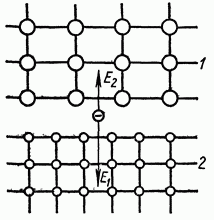
\includegraphics[width=0.3\textwidth]{1}
		\label{fig:pic1}
		\vspace{-10pt}
		\caption{Граница поверхности двух разных металлов}
	\end{wrapfigure}
	
	\subsection{Вклад различия работы выхода}
	На электроны, оказавшиеся в пограничной области, со стороны металла \textbf{1} действуют меньшие силы, чем со стороны металла \textbf{2}, имеющего более плотную ионную решетку; работа выхода электрона из металла \textbf{1} будет меньше, чем из металла \textbf{2}. Положим, что металлы посылают одинаковое число электронов $n_1 = n_2$; из этих электронов большая часть втягивается в металл \textbf{2}. Таким образом, первый заряжается положительно, второй — отрицательно. Это вызовет появление в пограничной области внешнего электрического поля, которое будет препятствовать такому переходу электронов. Со временем наступает равновесие. 
	
	Поскольку поля \textbf{E$_1$} и \textbf{E$_2$} противоположны по направлению, модуль суммарного поля \textbf{E} будет равен
	$$E = E_1 - E_2$$ Если это выражение умножить на $dx$ и проинтегрировать, то получим \begin{equation}
	(\phi_1 - \phi_2)_A = -(A_1 - A_2)/e
	\label{eq1}
	\end{equation}, где $A_1$ и $A_2$ -- работы выхода электрона из металлов \textbf{1} и \textbf{2} соответственно, а $e$ -- заряд электрона (знак 'минус' учитывает направление векторов).
	
	\subsection{Вклад различия плотностей электронного газа}
	Пусть теперь у металлов равны работы выхода, но $n_1 \ne n_2$. Для простоты положим, что в любой точке \textbf{E$_1$} и \textbf{E$_2$} уравновешивают друг друга. В следствие диффузии электронов на границе возникнет электрическое поле и, следовательно, разность потенциалов. При этом в состоянии равновесия работа по переходу электрона против установившейся разницы потенциалов будет $A = e(\phi_1 - \phi_2)$. Более того, из распределения Гиббса для энергии имеем:
	$$ n_2 = n_1 \exp\left(\frac{-\Delta A}{kT}\right)$$
	Тогда
	\begin{equation}
	(\phi_1 - \phi_2)_n \equiv \frac{\Delta A}{e} = \frac{kT}{e} \ln\frac{n_1}{n_2}
	\label{eq2}
	\end{equation}
	
	Если действуют оба вклада, то разница потенциалов:
	\begin{equation}
	\phi_1 - \phi_2 = - \frac{A_1 - A_2}{e} + \frac{kT}{e} \ln\frac{n_1}{n_2}
	\label{finEq}
	\end{equation}
	
	\section{Эффект Пельтье}
	Если теперь через пограничную область пропустить электрический ток, то электроны, проходя через эту область, будут в зависимости от направления тока либо ускоряться, либо тормозиться от контактного поля. В первом случае в пограничном слое наблюдается выделение тепла (электроны, получившие кинетическую энергию, будут при столкновениях передавать энергию атомам металла); во втором случае — поглощение тепла (электроны, потерявшие скорость, будут
	при столкновениях с атомами получать от них энергию, т. е. охлаждать металл). Выделение или поглощение тепла при прохождении тока через пограничную область, обусловленное работой контактного электрического поля называется эффектом Пельтье.
	
	При прохождении тока изменение теплоты составит (с учетом того, что $(\phi_B)_A - (\phi_C)_A = 0$):
	\begin{equation}
	\Delta Q = (\phi_B - \phi_C) It = (\phi_1 - \phi_2)_n It = \left(\frac{kT}{e} \ln \frac{n_1}{n_2}\right) It
	\label{peEq}
	\end{equation}
	Здесь мы не учли вклад разности работы выхода, поскольку мы имеем дело 
	\section{Практическое применение эффекта Пельтье}
	Эффект Пельтье используется там, где необходимо охлаждение, но затруднено использование холодильных установок со фреоном. Основанные на нем элементы имеют малый КПД, поэтому они не годятся для получения больших разниц температур. Элементы Пельтье используются в автомобильных холодильниках (поскольку в них использование полноценных компрессоров затруднительно), а также в системах охлаждения плат. При этом КПД таких установок составляет $5-8\%$.
\bibliography{mybibliography}
\bibliographystyle{gost705}
\end{document}